\documentclass[aspectratio=169]{beamer}
\usepackage[utf8]{inputenc}
\usepackage[T1]{fontenc}
\usepackage{graphicx}

\title{title of the presentation​​}
\author[name1, name2, name3]{name1*, name2 and name3}
\date[site]{site and date}

% UofC theme
% style should be one of
% simple, bold, flourish or conservative
% miniframes adds a navigation bar on top
%\usetheme[style=simple]{uofc}
\usetheme[style=bold]{uofc}
%\usetheme[style=bold,miniframes]{uofc}
%\usetheme[style=flourish]{uofc}
%\usetheme[style=conservative]{uofc}

\begin{document}

\begin{frame}
 \titlepage 
\end{frame}

\section{Introduction}
\begin{frame}
 \frametitle{Frame title}
 Hello world!\\
 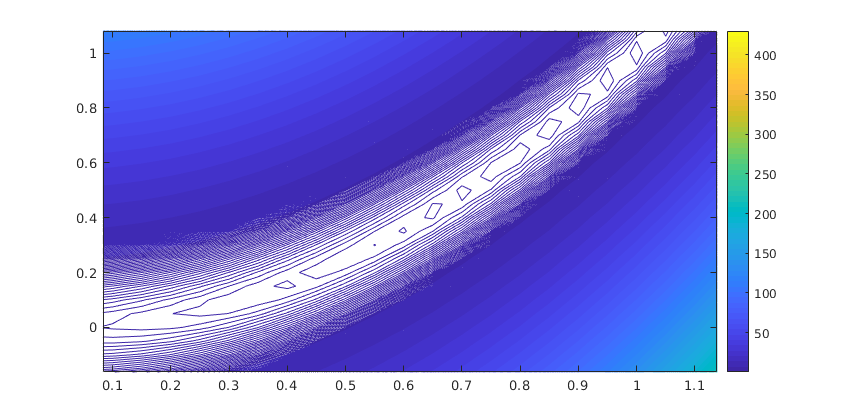
\includegraphics[scale=0.5]{images/rosenbrockzoom.png}\\
 Description of the image.
\end{frame}

\begin{frame}
 \frametitle{Frame title }
 Hello world!\\
 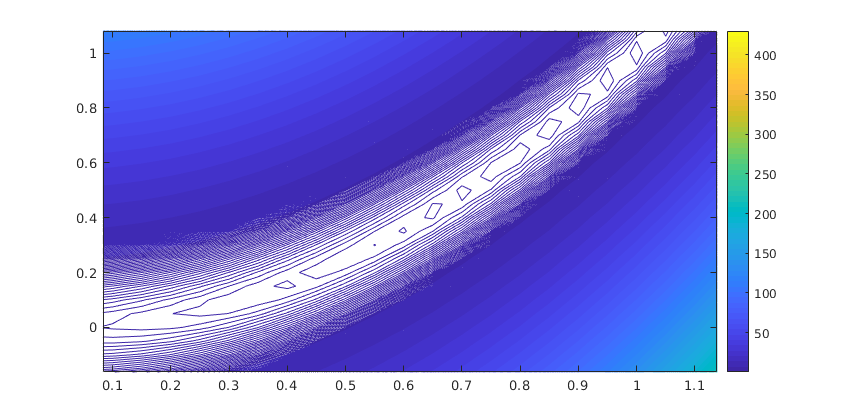
\includegraphics[scale=0.5]{images/rosenbrockzoom.png}\\
 Description of the image.
\end{frame}

\section{Theory}
\begin{frame}
 \frametitle{Frame title }
 Hello world!\\
 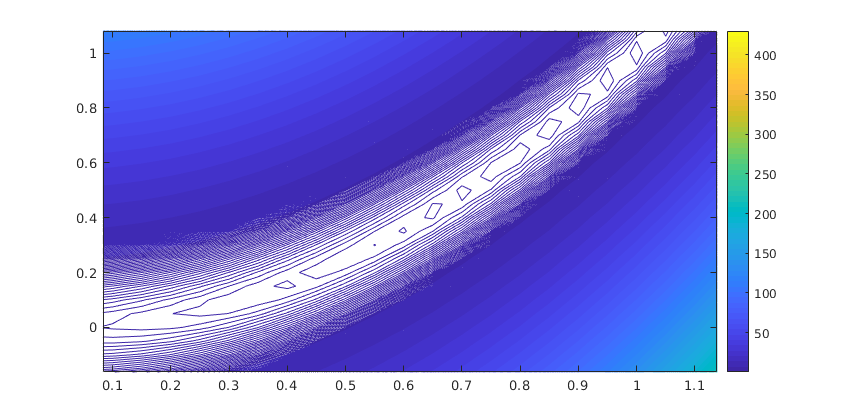
\includegraphics[scale=0.5]{images/rosenbrockzoom.png}\\
 Description of the image.
\end{frame}

\section{Results}
\begin{frame}
 \frametitle{Frame title }
 Hello world!\\
 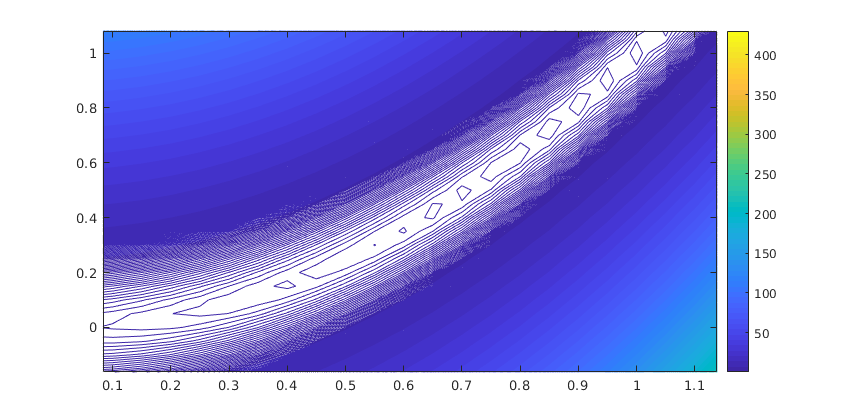
\includegraphics[scale=0.5]{images/rosenbrockzoom.png}\\
 Description of the image.
\end{frame}

\section{Discussion}
\begin{frame}
 \frametitle{Frame title }
 Hello world!\\
 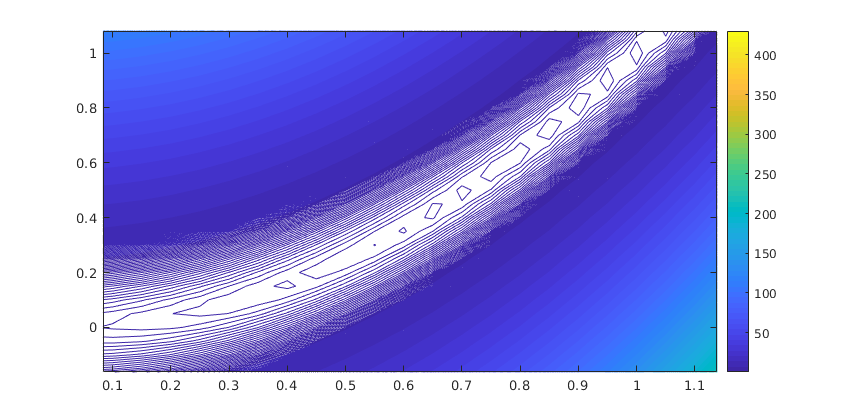
\includegraphics[scale=0.5]{images/rosenbrockzoom.png}\\
 Description of the image.
\end{frame}

\end{document}
